\section{Embedded RT Systems}
\subsection{Definition Embedded Systems}
Ein Embedded System \ldots
\begin{itemize}
  \item \ldots ist ein System, das einen Computer beinhaltet, aber keiner ist
  \item \ldots besteht üblicherweise aus HW und SW
  \item \ldots ist häufig ein Control System
\end{itemize}
\subsubsection{Charakterisierung von Embedded Systems}
Embedded Systems können (müssen aber nicht) folgende Eigenschaften haben:
\begin{itemize}
  \item \textbf{Reaktive Systeme} : Interagieren mit ihrer Umgebung
  \item \textbf{Echtzeitsysteme/Real-time systems} : Definierbare zeitliche
        Anforderungen erfüllen
  \item \textbf{Verlässliche Systeme/Dependable systems}: Sehr hohe
        Zuverlässigkeitsanforderungen erfüllen
  \item \textbf{Weitere Anforderungen/Charakteristiken}:
        \begin{itemize}
          \item Kleiner Energieverbrauch
          \item Kleine physikalische Abmessungen
          \item Lärm, Vibration, Feuchtigkeit etc.
        \end{itemize}
\end{itemize}

\subsubsection{Deeply Embedded System}
Ein Deeply Embedded System \ldots
\begin{itemize}
  \item \ldots ist ein Embedded System mit minimaler Benutzerschnittstelle, üblicherweise ohne GUI und ohne Betriebssysstem
  \item \ldots beschränkt sich auf eine Aufgabe wie z.B. die Regelung eines physikalischen Prozesses
  \item \ldots muss sehr oft zeitliche Bedingungen erfüllen (Echtzeitsystem)
\end{itemize}

\subsubsection{Betriebssysteme bei Embedded Systems}
\begin{itemize}
  \item Betriebssysteme wie (Embedded) Linux und Android können zum Einsatz kommen
        \begin{itemize}
          \item Achtung: Linux und Android sind nicht echtzeitfähig!
        \end{itemize}
  \item Wenn Echtzeit verlangt wird, kommen oft \textbf{Echtzeit-Betriebssysteme (Real-time operating system, RTOS)} zum Einsatz
\end{itemize}

\subsubsection{Bare Metal Embedded System}
\begin{itemize}
  \item Bei einem \textbf{Bare Metal Embedded System} kommt keinerlei Betriebssystem zum Einsatz
        \begin{itemize}
          \item insbesondere bei Deeply Embedded Systems recht häufig
        \end{itemize}
\end{itemize}

\subsubsection{Verfügbarkeit (Availability)}
Anteil an der Betriebsdauer, in  der das System seine Funktion
erfüllt:

\begin{equation}
  Verfuegbarkeit = \frac{Gesamtzeit-Ausfallzeit}{Gesamtzeit}
\end{equation}

\subsection{Definition Real-time Systems}
\textbf{Definition:} System, das Informationen innerhalb einer definierten Zeit
(deadline) bearbeiten muss. Es erfüllt explizite Anforderungen an die
Antwortzeiten.\\
\textbf{Antwortzeit:} Zeit vom Stimulus (Vorhandensein
Eingangswert) bis zum Erscheinen des Ausgangswerts\\
{\centering
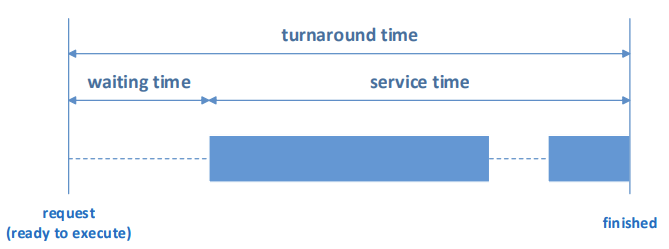
\includegraphics[height=3cm]{images/RTSystems/Task_Zeitdef.png}\\}
Antwortzeit (response time, turnaround time) =  Wartezeit (waiting time) + Bearbeitungszeit (service time)\\
\textbf{Fehlerhaftes System:} Es werden nicht alle formal definierten Systemspezifikationen erfüllt.
Es muss sowohl der Output wie auch die Einhaltung der zeitlichen Anforderungen stimmen\\
\textbf{Soft real-time system:} System wird durch das Verletzen von
Antwortzeiten nicht ernsthaft beeinflusst $\rightarrow$ Komforteinbussen (Bsp.:
Geldautomat)\\
\textbf{Firm real-time system:} Durch Verletzen weniger Antwortzeiten wird das
System nicht ernsthaft beeinflusst. Bei vielen Verletzungen jedoch $\rightarrow$
kompletter Ausfall, katastrophales Fehlverhalten (Bsp.: GPS-gesteuerter
Rasenmäher)\\
\textbf{Hard real-time system:} Durch Verletzen der Antwortzeiten wird das
System ernsthaft beeinflusst $\rightarrow$ kompletter Ausfall, katastrophales
Fehlverhalten (Bsp.: Helikoptersteuerung)\\
\textbf{Determinismus:} Für jeden möglichen Zustand und alle möglichen
Eingabewerte sind jederzeit der nächste Zustand und die Ausgabewerte definiert.

\begin{multicols}{2}
  \textbf{Auslastung/Utilization}:
  Auslastung pro Prozess:
  \begin{center}
    \begin{tabular}{c c}
                                                   & $u_\text{i}$ = Auslastungsfaktor des Tasks i \\
      $u_\text{i} = \frac{e_\text{i}}{p_\text{i}}$ & $e_\text{i}$ = Executionzeit des
      Tasks i                                                                                     \\
                                                   & $p_\text{i}$ = Executionperiode des Tasks i
    \end{tabular}\\
  \end{center}

  \columnbreak

  Für n periodische Tasks erhalten wir die gesamte Auslastung U:
  \begin{center}
    \begin{equation}
      U = \sum_{i=1}^{n}u_\text{i} = \sum_{i=1}^{n}\frac{e_\text{i}}{p_\text{i}}
    \end{equation}
  \end{center}
\end{multicols}
